% !TeX encoding = UTF-8
% !TeX spellcheck = en_US

\documentclass[
	paper=A4,
	parskip=full,
	chapterprefix=true,
	11pt,
	headings=normal,
	bibliography=totoc,
	listof=totoc,
	titlepage=on,
]{scrreprt}

\usepackage{../../lieb}

\usepackage{feynmp}
\DeclareGraphicsRule{.1}{mps}{*}{}

\graphicspath {{../images/}}

\heads{RWTH Aachen \\ Particlephyics Lab}{T13 \\ Paul Trap}{Lieb | Stettner \\ \today} 
\date{\today}

\newcommand{\thirdwidth}{0.32\textwidth}
\newcommand{\halfwidth}{0.48\textwidth}
\newcommand{\fullwidth}{1.0\textwidth}

\setlength\parindent{0pt}
\setlength{\parskip}\medskipamount

\title{Particle Physics Laboratory Class \\ \quad \\ Experiment T13 | Paul Trap }
\author{Jonas Lieb (312136) \\ Jöran Stettner (312169) \\ \\  RWTH Aachen}



\begin{document}

\maketitle

\cleardoublepage

\setcounter{tocdepth}{2}
\tableofcontents

\cleardoublepage

\chapter{Introduction and Theory}

In this laboratory report, the storage of charged particles and a measurement of their specific charge is presented. The experiment consists of a Paul trap, named after its creator Wolfgang Paul, which constrains the movement of ionized aluminum powder particles to stable trajectories by applying three alternating electrical fields. 

\section{Trapping Particles in Electrical Fields}

Beside the storage of charged particles by B-fields, it is possible to trap particles in electrical fields. In a static electrical field of arbitrary shape, the particle will follow the field lines and finally hit the source of the field (e.g. the capacitor plate) or diverge (e.g. field of charged sphere). However, with time dependent fields it is possible to create an electrical potential having a minimum when averaged over time. If the frequency of these fields is larger than the movement of the particle, a stable trajectory exists and the particle gets trapped. \\

In a cubic geometry (6 plates, opposing plates at same potential), the following equation of motion holds for all three dimensions. In this so called Mathieu equation, the index $i$ stands for the three spatial components, $\Omega$ is the frequency of the alternating fields, $\xi = \frac{1}{2} \Omega t$ is the normalized time and $a_i, q_i$ are constants depending on the applied voltages and the particle's properties.
\begin{equation}
\label{eq:mathieu}
\left(a_i+q_i \cos(2 \xi)\right) x_i + \frac{d^2x_i}{d\xi^2} = 0
\end{equation}

The full solution of this equation is discussed elsewhere (e.g. in the lab manual\cite{Lab_manual}), only the following aspects are important for the conducted experiment.

\subsection{Stability of the Particle Trajectories}
The exact solution for the particle trajectories can be expressed as an infinite series. However, the tracks are only finite under certain conditions. Depending on the applied alternating field $U_i$ and the constant field $U'$ (same potential on both plates), the constants $a$ and $q$ change. The constants in x-direction are given in equation \ref{eq:a} and \ref{eq:q}, where $K$ is a geometry factor of the plates, $m$ the mass of the particle, $q$ the charge of the particle and $r_0$ the distance of the plates to the center.
\begin{equation}
	\label{eq:a}
	a_x=\frac{16 K q}{3 \Omega^2 m r_0^2} U'
\end{equation}
\begin{equation}
	\label{eq:q}
	q_x= \frac{-4 K q}{ \Omega^2 m r_0^2} U_{x}
\end{equation}

For stable trajectories, the voltages have to be adjusted such that the following equation holds\cite{Lab_manual}:
\begin{equation}
	\label{eq:beta}
	\beta_x  = \sqrt{a_x+\frac{q_x^2}{2}}  \in (0,1)
\end{equation}
Additionally, air friction helps to stabilize the particle tracks since it damps the motion (Stokes' term in the Mathieu equations leads to weaker conditions). 

\subsection{Influence of an Additional Force in z-Direction}
Instead of applying an additional potential to both x-plates, it is also possible to apply an additional static electrical field in z-direction (homogeneous, pointing upwards, different potential on the plates). The idea is to compensate the gravitational force which acts on the particle. If considered in the Mathieu equations, a net force in z-direction does not change the shape of the particle tracks but shifts the center of the trajectories. However, if the applied field compensates the gravitational force, there is no shift of the particles and the particle tracks become independent of the applied alternating focusing voltage $U_z$ \cite{Lab_manual}.

\subsection{Influence of an Additional Alternating Field in x-Direction}

As a third option, the influence of an additional alternating field in x-direction is discussed. While the alternating fields $U_i$ have same potential on opposing plates, the field $U_W$ acts homogeneously in x-direction (different potential on opposing plates). The additional term in the Mathieu equation leads to modified trajectories: The particle shakes back and forth. By changing the driving frequency of the field $U_W$ resonances can be observed (forced, damped harmonic oscillator with damping constant $k_L$ from the Stokes' term describing air friction):
\begin{equation}
\omega_W^{res} = \frac{\Omega}{2} \sqrt{\beta_x^2 - 2 k_L^2}
\end{equation}


\chapter{Experimental Setup}

The trap consists basically of 6 copper rings and a high voltage source, see figure \ref{fig:trap}. The rings are arranged in a cubic geometry: Each two rings facing each other lie on the same potential. The amplitude of the focusing voltages $U_x$, $U_y$ and $U_z$ can be adjusted individually, but the phase between them remains $\SI{120}{\degree}$. Additionally, a lamp and a camera are used to illuminate and observe the trapped particles inside the trap (not visible on the picture). To inject a few particles of aluminum powder, a syringe is installed below the trap. By pressing it, the particles are pushed upwards and become charged by the friction with the surrounding material of the syringe or air. 
\begin{figure}
	\centering
	\begin{subfigure}[t]{0.4\textwidth}
		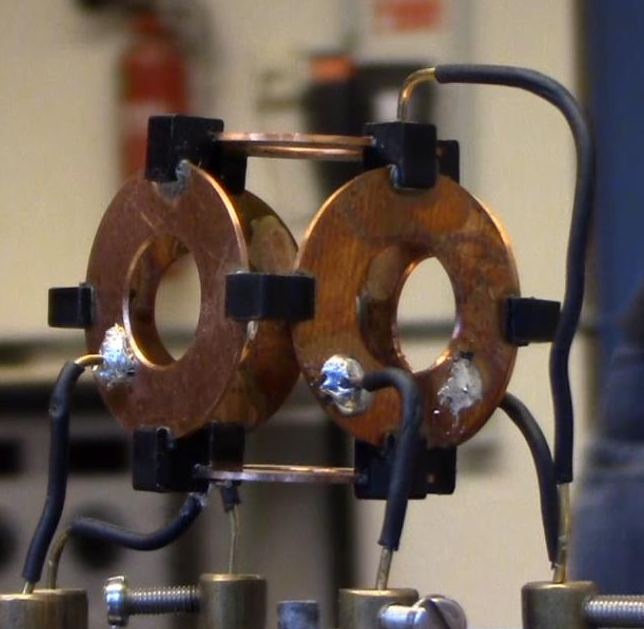
\includegraphics[width=0.9\textwidth]{capture_20150916_124003_cut}
		\caption{Picture of the Paul Trap during installation. The 6 copper rings are connected to a three phase high voltage supply.}
		\label{fig:trap}
	\end{subfigure}	
	\begin{subfigure}[t]{0.4\textwidth}
		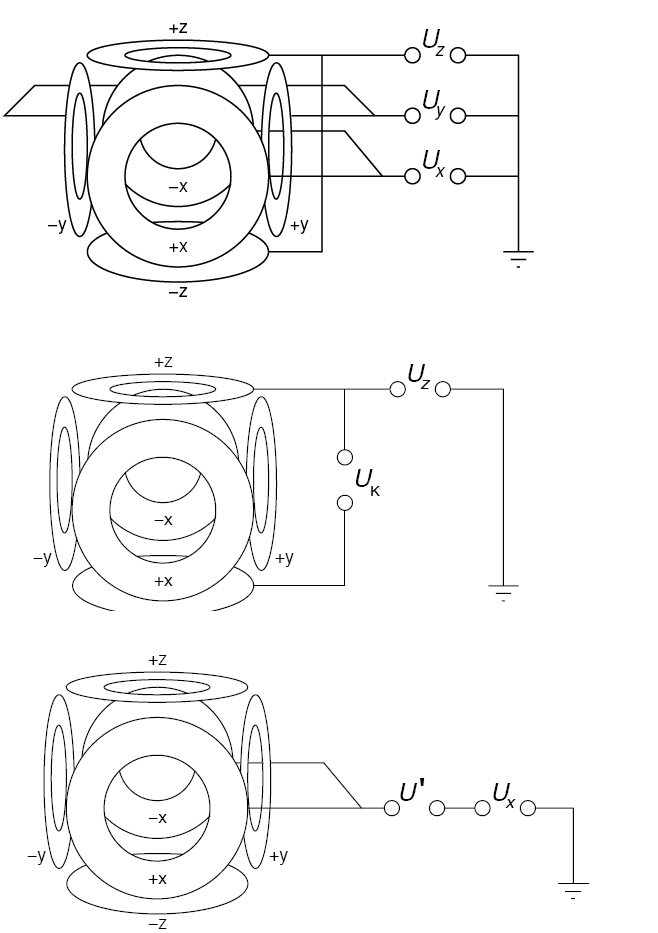
\includegraphics[width=0.9\textwidth]{Circuits}
		\caption{Sketches of the electrical circuits for the additional applied voltages, taken from \cite{Lab_manual}.From top to bottom: The circuits of the alternating fields with phase difference $\SI{120}{\degree}$, the constant field in upwards z-direction and the constant potential which can be applied to the x-rings.}
		\label{fig:circuits}
	\end{subfigure}
\caption{The experimental setup.}
\end{figure}

Furthermore, three additional voltages can be applied to some rings of the trap (electrical circuits are shown in figure \ref{fig:circuits}) : 
\begin{itemize}
	\item An additional direct voltage to the two rings in x-direction: $U'$ (same potential on both x-rings)
	\item A direct voltage in between the two z-rings creating a constant electrical field upwards in z-direction (different potential on the two z-rings): $U_K$
	\item An overlayed alternating voltage on both x-rings (different potential) creating an alternating field in x-direction: $U_W$
\end{itemize}


The second stage of the experimental setup consists of a similar trap and the same electrical circuits, but enclosed in a cylinder. A two-stage vacuum pump is connected to the cylinder and creates a low-pressure environment down to ($p \approx \SI{5}{\micro \bar}$). The vacuum is monitored by a pressure sensor.

\chapter{Conduction and Analysis}
\label{ch:analysis}
In the following chapter, the conducted experiments and their results are reported. Each measurement is repeated in a low pressure environment to investigate the influence of air friction on the trapped particles. Since the particle trajectories are much more instable without air friction, the low pressure cylinder is not evacuated to the lowest limit of the vacuum pump, but operated once at $p = \SI{300}{\milli \bar}$ and once at $p = \SI{150}{\milli \bar}$. \\
Each conducted measurements yields a value of the specific charge $\frac{q}{m}$ which is different for the aluminum particles because their size and their acquired charge differ. To compare the different methods, the measurements are conducted in a series with the same trapped particle.\\
As discussed in chapter \ref{ch:systematics}, the output of the high voltage source does not match its adjusted values. The following correction factors are therefore applied to all adjusted voltages and will be justified later:

\begin{table}[htbp]
	\centering
	\begin{tabular}{ 
			l
			S[table-format=1.2(2)]
		}
		\toprule
		{Voltage} & {Correction Factor} \\ 
		\midrule
		$U_x$ & 0.78 +- 0.02  \\
		$U_y$ & 0.76 +- 0.03 \\
		$U_z$ & 0.81 +- 0.03 \\
		$U_K$ and $U'$ & 0.61 +- 0.01 \\
		$U_W$ & 0.17 +- 0.03 \\
		
		\bottomrule
	\end{tabular}
	\caption{Correction factors to compensate for the mismatching output of the voltage source. The determination of these factors is described in chapter \ref{ch:systematics}.}
	\label{tbl:corr_factors}
\end{table}


\section{Measurement I - Stability of the Trajectories}
In this measurement, the charge-mass ratio $\frac{q}{m}$ is determined using the stability boundaries $\beta = 0$ from equation \ref{eq:beta}.

The electric fields $U_i$ are adjusted to different values between \SIrange{500}{100}{\volt}, setting the displayed voltages equal on each step $U_x = U_y = U_z$. Starting at $U' = 0$, the additional direct voltage on the rings in x-direction is increased until the observed particle track appears unstable.

Due to the fluctuation of $U'$ and the necessity to keep the particle inside the trap for the two subsequent measurements, the instability criterion has been chosen conservatively: A track is classified as unstable if any part of the track leaves the observation area visible through the ring facing the camera (figure \ref{fig:stability_example}).
\begin{figure}
	\centering
	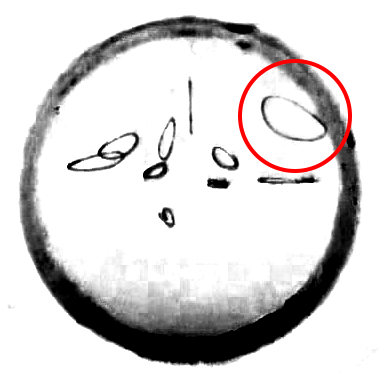
\includegraphics[width=0.4\textwidth]{stability_example}
	\caption{Example for the stability measurement. The highlighted particle track on the upper right side has shifted to the edge of the visible area and is thus classified as unstable. The image has been cropped and the colors inverted to increase readability.}
	\label{fig:stability_example}
\end{figure}

From the recorded values $U_x, U'_\mathrm{crit}$ and $\Omega$, the charge-mass ratio can be calculated as follows:
\begin{equation}
	\frac{q}{m} = -\frac{2}{3} \cdot \frac{r_0^2 \ \Omega^2}{K} \cdot \frac{U'_\mathrm{crit}}{U_x^2}
\end{equation}
This measurement primarily yields the last term $a \defeq U_\mathrm{crit}' / U_x^2$. It is obtained by a linear regression over multiple values at various $U_x$. 
The assumed errors are discussed in detail in chapter \ref{ch:systematics}, relevant for the linear regression are the statistical uncertainties on $U'$ and $U_x$.
The linear regression is performed as a $\chi^2$-minimization on the function $f(x) = a\ x$. To estimate the parameter error, the linear regression is repeated \num{1000} times. Each time, the values for $x'$ and $y'$ are chosen from a normal distribution of width $\sigma_x$ ($\sigma_y$) around $x$ ($y$). The standard deviation on all fit results is taken as final uncertainty on the parameter.

The error on the slope is obtained by simulating \num{100} experiment outcomes within the data points' uncertainties.




, as well as an uncertainty of \SI{1}{\hertz} on the frequency measurement. The error on $K$ is neglected.


\section{Measurement II - Application of an Additional Field in z-Direction}
\section{Measurement III - Resonance Study}

\chapter{Uncertainties}
\label{ch:systematics}
\section{High Voltage Source}
\subsection{Mismatch of the Internal Voltage Measurement}
The high voltage source displays the adjusted voltage. However, a cross-check measurement with a multimeter shows discrepancies for all voltages of the source. To account for this, correction factors have been introduced in chapter \ref{ch:analysis}. They were determined by adjusting four different voltages, measuring them with the multimeter and comparing them to the displayed values. The ratio of the measured and adjusted values is averaged and the standard deviation is computed. The results are shown in table \ref{tbl:corr_factors} and are used in the analysis as correction factors. The systematic uncertainty which arises from the uncertainty on these correction factors is negligible compared to other uncertainties which are discussed in the following.

\subsection{Fluctuations of the Voltage Source}
The displayed voltage values on the voltage source fluctuate strongly. To read-off a voltage value, approximately four subsequent values are averaged live during the adjustment. The uncertainties arising from this can be estimated as follows: A longer set of voltage values is recorded ($N\approx20$) and the difference of the mean in subsamples of four is investigated. The standard deviation of the means from the subsamples gives an estimator for the fluctuation. This simulates the read-off process and yields the following uncertainties on the voltage values:

\begin{table}[htbp]
	\centering
	\begin{tabular}{ 
			l
			S[table-format=2]
		}
		\toprule
		Voltage & {Uncertainty [$\si{\volt}$]} \\ 
		\midrule
		$U_x$ & 11  \\
		$U_y$ & 12 \\
		$U_z$ & 6 \\
		$U_K$ and $U'$ & 16 \\
		$U_W$ & 8 \\
		
		\bottomrule
	\end{tabular}
	\caption{Uncertainties on the adjusted voltage values arising from the fluctuating display of the voltage source.}
	\label{tbl:unc_fluctuation}
\end{table}

\section{Evauluation of the Track Stability}
During Measurement II, the constant voltage $U'$ is increased until the particle trajectory becomes instable. However, the point of instability can be determined only to a precision of roughly $10\%$: The trajectory could as well be called instable if $U'$ is increased or decreased in this range. 
 
\section{Frequency of the Alternating Fields}
The frequency of the alternating fields which is displayed on the voltage source can not be cross-checked in this setup. However, there is still a fluctuating which can be taken into account: The adjusted frequency fluctuates in the range of $\pm \SI{1}{\hertz}$. This uncertainty is treated in all analysis steps as statistical. 

\section{Distance Measurements}
The distance $r_0$ from the rings to the center of the trap is used in all analysis steps. It is determined with a sliding caliper between opposing rings. The uncertainty (difference between $r_0$ in x,y or z-direction) is $\sigma_{r_0} \approx \SI{0.5}{\milli \meter}$. The influence of this uncertainty is negligible compared to other discussed uncertainties. The same holds for the measurements of the ring diameter which is used to find the scale for the oscillation amplitude in measurement III.

\chapter{Comparison of Results}


\cleardoublepage

\bibliographystyle{utphys}
\bibliography{T13_bib}{}

\end{document}


